\section{Metodologia Adotada}

Neste trabalho, pretende-se modificar e desenvolver novas aplicações. Além disso, integrá-las e validá-las através de experimentos no PIS localizado na UFES no Laboratório de Visão Computacional e Robótica.

Para integrar dispositivos robóticos dentro do PIS, faz-se necessário adicionar o sistema embarcado que os controlam dentro da plataforma de orquestração de contêineres como nós de computação em borda. Assim, obtendo um \textit{cluster} formado por nós de computação em nuvem (\textit{Datacenter} presente no laboratório) e nós de computação em borda.

Para isso, pretende-se utilizar uma Raspberry 4B, como exemplo de dispositivo para computação em borda. Ao integrá-la \add{ao} \textit{cluster} Kubernetes já existente no laboratório, pretende-se variar a largura de banda da conexão disponível com a nuvem. Dessa forma, ao orquestrar as aplicações no \textit{cluster}, pretende-se analisar as informações multiníveis disponibilizadas pelas ferramentas de observabilidade presentes no PIS e desenvolver um controlador responsável por avaliar onde as aplicações devem ser executadas, em nuvem ou em borda, a fim de atender os requisitos das aplicações com utilização racional dos recursos de infraestrutura.

É importante notar que, para \recom{ser possivel}{se} obter as informações desejadas, é necessário que as aplicações sejam instrumentadas corretamente. Ou seja, é necessário modificar as aplicações inserindo blocos de códigos responsáveis por enviar as informações desejadas, tais como tempo de resposta.

\begin{figure}[ht]
    \centering
    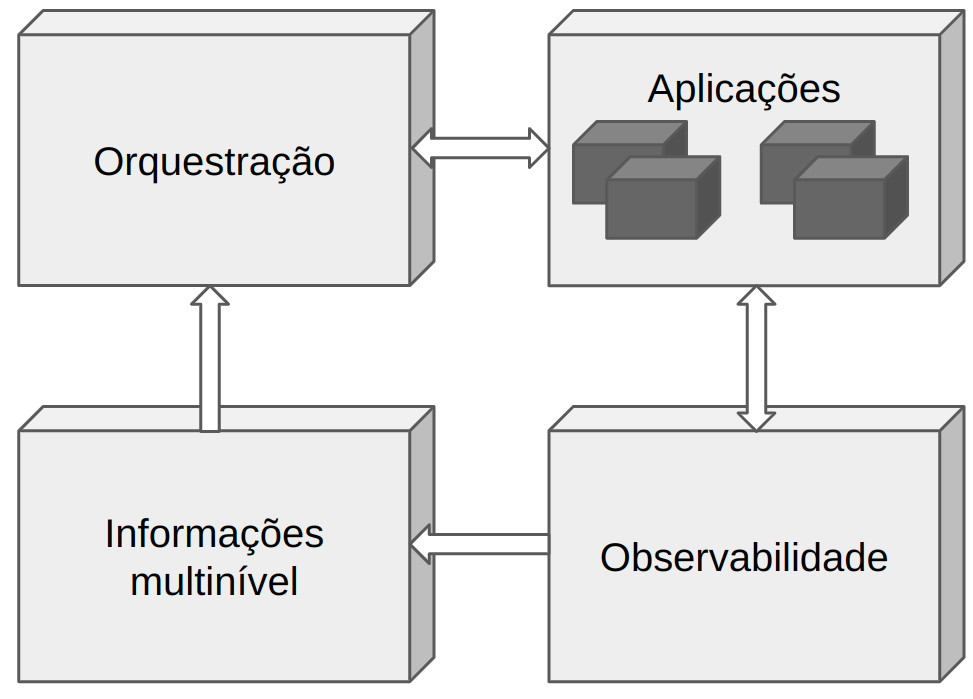
\includegraphics[width=80mm]{images/metodologia.png}
    \caption{Metodologia adotada.}
    \label{fig:metodologia}
\end{figure}


Na Figura \ref{fig:metodologia}, pode-se observar como \recom{pretende-se}{se pretende} realizar este trabalho. Tanto as aplicações quanto as ferramentas de observabilidade se comunicam a fim de mensurar as informações desejadas. Por sua vez, as ferramentas de observabilidade disponibilizam essas informações para o PIS, tanto informações características das aplicações, como o tempo de resposta, quanto informações da infraestrutura, como o uso de CPU e memória. A partir dessas informações, pretende-se desenvolver um controlador integrado à plataforma de orquestração de contêineres para alocar corretamente as aplicações.

\section{Cronograma de Trabalho}

O trabalho será desenvolvido conforme as etapas apresentadas a seguir.

\begin{itemize}
\item 
\textbf{Atividade 1. Revisão bibliográfica}:
(\textit{i}) estudo sobre computação em borda e espaços inteligentes;
(\textit{ii}) revisão a respeito das técnicas para computação em borda no contexto de Espaços Inteligentes.

\item 
\textbf{Atividade 2. Criar e configurar uma plataforma para computação em borda e em nuvem}:
(\textit{i}) criar uma plataforma de orquestração de contêineres com dispositivos robóticos como nós de computação em borda e servidores como nós de processamento em nuvem;
(\textit{ii}) configurar a plataforma.

\item 
\textbf{Atividade 3. Instalar as aplicações de suporte ao PIS}:
(\textit{i}) realizar a instalação dos softwares que compõe o PIS e configurar a integração entre nuvem e borda.

\item 
\textbf{Atividade 4. Adaptação das aplicações do sistema}:
(\textit{i}) adaptação das aplicações que irão compôr o sistema para expôr o tempo de resposta total;
(\textit{ii}) construção das imagens de contêineres para execução em borda e em nuvem;

\item 
\textbf{Atividade 5. Desenvolvimento de um controlador para realizar o gerenciamento das aplicações}:
(\textit{i}) determinação do tempo de resposta total em borda e em nuvem;
(\textit{ii}) desenvolver um controlador responsável por decidir onde orquestrar as aplicações (em nuvem ou em borda) com base no tempo de resposta;
(\textit{ii}) escrever a documentação do controlador;

\item 
\textbf{Atividade 6. Validação do controlador desenvolvido}:
(\textit{i}) realizar experimentos variando a largura de banda disponível em borda e verificar como o controlador orquestra as aplicações;
(\textit{ii}) gerar gráficos e apresentar resultados do sistema em funcionamento.

\item 
\textbf{Atividade 7. Redação do projeto de graduação}:
(\textit{i}) expandir o referencial teórico;
(\textit{ii}) descrever a arquitetura do sistema;
(\textit{iii}) apresentar e discutir os resultados.

\item 
\textbf{Atividade 8. Revisão do projeto de graduação}:
(\textit{i}) revisar o texto junto à orientadora e coorientador;
(\textit{ii}) corrigir os possíveis erros.

\item 
\textbf{Atividade 9. Defesa do projeto de graduação}:
(\textit{i}) após a aprovação da escrita, a defesa do projeto de graduação será realizada.

\end{itemize}

%1. DEFINIMOS O NUMERO DE MESES NOS QUAIS SERÁ IMPLEMENTADO O PROJETO
\newcommand{\DuracionPlanoMeses}{6}

% 2. DEFINIMOS AS ATIVIDADES COMO COMANDOS VIA \newcommand{\name_comand}{value}
% primeira atividade
\newcommand{\AtvAlgRotI}{Revisão bibliográfica}
% segunda atividade
\newcommand{\AtvAlgRotII}{Criar e configurar uma plataforma para computação em borda e em nuvem}
% terceira atividade
\newcommand{\AtvAlgRotIII}{Instalar as aplicações de suporte ao PIS}
% quarta atividade
\newcommand{\AtvAlgRotIV}{Adaptação das aplicações do sistema}
% quinta atividade
\newcommand{\AtvAlgRotV}{Desenvolvimento de um controlador para realizar o gerenciamento das aplicações}
% sexta atividade
\newcommand{\AtvAlgRotVI}{Validação do controlador desenvolvido}
% setima atividade
\newcommand{\AtvAlgRotVII}{Redação do projeto de graduação}
% oitava atividade
\newcommand{\AtvAlgRotVIII}{Revisão do projeto de graduação}
% nona atividade
\newcommand{\AtvAlgRotIX}{Defesa do projeto de graduação}


% 3. DEFINIMOS OS ROTULOS DAS AS ATIVIDADES A SER USADAS NO DIAGRAMA DE GANTT USANDO O COMANDO \newcommand{\name_comand}{value}
%ROTULOS DE ATIVIDADES
\newcommand{\RTLAtvAlgRotI}{ATV 1} %rotulo da primeira atividade
\newcommand{\RTLAtvAlgRotII}{ATV 2} %rotulo da segunda atividade
\newcommand{\RTLAtvAlgRotIII}{ATV 3} %rotulo da terceira atividade
\newcommand{\RTLAtvAlgRotIV}{ATV 4} %rotulo da quarta atividade
\newcommand{\RTLAtvAlgRotV}{ATV 5} %rotulo da quinta atividade
\newcommand{\RTLAtvAlgRotVI}{ATV 6} %rotulo da sexta atividade
\newcommand{\RTLAtvAlgRotVII}{ATV 7} %rotulo da sétima atividade
\newcommand{\RTLAtvAlgRotVIII}{ATV 8} %rotulo da oitava atividade
\newcommand{\RTLAtvAlgRotIX}{ATV 9} %rotulo da nona atividade


%4. COMENTARIOS SOBRE O DIAGRAMA DE ATIVIDADES
Apresenta-se nesta seção uma previsão do cronograma do plano de trabalho. Esse projeto será realizado no período correspondente ao semestre 2023/2, aproximadamente \DuracionPlanoMeses\ meses. A data de início do projeto será 21 de julho de 2023 e a data prevista para encerramento, 16 de dezembro de 2023. Na Tabela \ref{Tab1}, são detalhadas as atividades que se pretende realizar para o desenvolvimento do plano de trabalho. Assim, na primeira coluna da tabela são definidos os rótulos de cada atividade e na segunda coluna é feita uma descrição da atividade que se pretende realizar. Finalmente, na Figura \ref{fig:gaant-cronograma} é apresentado o diagrama de tempo das atividades indicadas na Tabela \ref{Tab1}.


%5. CRIAÇÃO DA TABELA DE ATIVIDADES, OBSERVE QUE AQUI SÃO USADOS OS COMANDOS DAS ATIVIDADES
\begin{table}[!htbp]
\begin{center}\begin{tabular}{c|p{13.50cm}}
\hline
Rótulo  & Atividade \\ 
\hline
\hline
\RTLAtvAlgRotI & \AtvAlgRotI \\ 
\hline 
\RTLAtvAlgRotII & \AtvAlgRotII \\ 
\hline 
\RTLAtvAlgRotIII & \AtvAlgRotIII \\ 
\hline
\RTLAtvAlgRotIV & \AtvAlgRotIV \\ 
\hline
\RTLAtvAlgRotV & \AtvAlgRotV \\
\hline
\RTLAtvAlgRotVI & \AtvAlgRotVI \\
\hline
\RTLAtvAlgRotVII & \AtvAlgRotVII \\
\hline 
\RTLAtvAlgRotVIII & \AtvAlgRotVIII \\
\hline 
\RTLAtvAlgRotIX & \AtvAlgRotIX \\
\hline 
\end{tabular}
\end{center}
\caption{
\footnotesize
Lista de atividades. 
}
\label{Tab1}
\end{table}

%6. CRIAÇÃO DO DIAGRAMA DE GANTT DAS ATIVIDADES, OBSERVE QUE AQUI SÃO USADOS OS COMANDOS DOS  ROTULOS DAS ATIVIDADES
\begin{figure}[!htbp]
\begin{center}
\begin{ganttchart}[
x unit = 0.55cm,
y unit title=0.5cm,
y unit chart=0.5cm,
hgrid,vgrid,
title label anchor/.style={below=-1.6ex},
title height=1,
bar/.style={fill=gray!50},
%group/.style={draw=black},
incomplete/.style={fill=white},
progress label text={},
bar height=0.7,
%group right shift=0,
group top shift=.6,
group height=.3,
group peaks width=.2]{1}{24}
%labels
\gantttitle{2023}{24}\\
\gantttitle{\tiny JUL}{4}
\gantttitle{\tiny AGO}{4} 
\gantttitle{\tiny SET}{4} 
\gantttitle{\tiny OUT}{4} 
\gantttitle{\tiny NOV}{4} 
\gantttitle{\tiny DEZ}{4}\\
%tasks

% Tercceira técnica
\ganttbar[bar/.style={fill=black},bar label font=\color{black}]{\RTLAtvAlgRotI}{1}{8} \\
\ganttbar[bar/.style={fill=black},bar label font=\color{black}]{\RTLAtvAlgRotII}{3}{4} \\
\ganttbar[bar/.style={fill=black},bar label font=\color{black}]{\RTLAtvAlgRotIII}{5}{6} \\
\ganttbar[bar/.style={fill=black},bar label font=\color{black}]{\RTLAtvAlgRotIV}{7}{8} \\
\ganttbar[bar/.style={fill=black},bar label font=\color{black}]{\RTLAtvAlgRotV}{9}{12} \\
\ganttbar[bar/.style={fill=black},bar label font=\color{black}]{\RTLAtvAlgRotVI}{13}{16} \\
\ganttbar[bar/.style={fill=black},bar label font=\color{black}]{\RTLAtvAlgRotVII}{5}{20} \\
\ganttbar[bar/.style={fill=black},bar label font=\color{black}]{\RTLAtvAlgRotVIII}{17}{20} \\
\ganttbar[bar/.style={fill=black},bar label font=\color{black}]{\RTLAtvAlgRotIX}{21}{22} \\

\end{ganttchart}
\end{center}
\caption{Diagrama de tempo das atividades a \recom{efetuar}{serem realizadas} para o desenvolvimento do plano de trabalho. }
\label{fig:gaant-cronograma}
\end{figure}